\documentclass{ximera}

\usepackage{float}

\newcommand{\R}{\mathbb R}

\newcommand{\href}[2]{#2\footnote{\url{#1}}}
\newcommand{\verticalvector}[1]{\begin{bmatrix}#1\end{bmatrix}}
\newcommand{\gt}{>}

\pgfplotsset{compat=1.8}
\graphicspath{
{./}
{introduction/}
{unit1/}
{unit1/theGeometryOfLinearEquations/}
{unit1/EliminationwithMatrices/}
{unit1/MultiplicationandInverseMatrices/}
}


\title{Factorization into A = LU}

\begin{document}
\begin{abstract}
  Unit 1 MIT OCW Linear Algebra: Factorization into A = LU
\end{abstract}
\maketitle

The MIT OCW Video Lecture can be found
here:\video{https://www.youtube.com/watch?v=5hO3MrzPa0A}\\

This session explains inverses, transposes and permutation matrices. We also learn how elimination leads to a useful factorization A = LU and how hard a computer will work to invert a very large matrix.

\begin{figure}[H]
\begin{image}
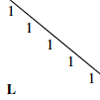
\includegraphics{1_4.jpg}
\end{image}
\end{figure}

One goal of today?s lecture is to understand Gaussian elimination in terms of matrices; to find a matrix $L$ such that $A = LU$. We start with some useful facts about matrix multiplication.

\section*{Inverse of a product}

The inverse of a matrix product $AB$ is $B_{?1} A_{?1}$.

\section*{Transpose of a product}

We obtain the transpose of a matrix by exchanging its rows and columns. In other words, 
the entry in row i column j of $A$ is the entry in row j column i of $A^T$.

The transpose of a matrix product $AB$ is $B^TA^T$. For any invertible matrix A, 
the inverse of $A^T$ is $(A^{-1})^T$

$A = LU$

We?ve seen how to use elimination to convert a suitable matrix $A$ into an upper 
triangular matrix $U$. This leads to the factorization $A = LU$, which is very helpful
in understanding the matrix $A$.

Recall that (when there are no row exchanges) we can describe the elimi�nation of the entries of matrix $A$ in terms of multiplication by a succession of elimination matrices $E_{ij}$, so that 
$A \rightarrow E21A  \rightarrow E_{31}E_{21}A  \rightarrow \cdots \rightarrow U$. In the two by two case this looks like:


\begin {table}[ht]
\centering
\begin {tabular} {c c c c}
$E_{21}$&$A$& &$U$\\
$\begin{bmatrix}  \phantom{-}1&0\\-4&1\end{bmatrix}$&$\begin{bmatrix} 2&1\\8&7\end{bmatrix}$&=&
$\begin{bmatrix} 2&1\\0&3\end{bmatrix}$
\end {tabular}
\end {table}

We can convert this to a factorization $A = LU$ by "canceling" the matrix $E_{21}$;
multiply by its inverse to get $E_{21}^{-1}E_{21}A = E_{21}^{-1}U$.

\begin {table}[ht]
\centering
\begin {tabular} {c c c c}
$A$& &$L$&$U$\\
$\begin{bmatrix} 2&1\\8&7\end{bmatrix}$&=&$\begin{bmatrix} 1&0\\4&1\end{bmatrix}$&
$\begin{bmatrix} 2&1\\0&3\end{bmatrix}$
\end {tabular}
\end {table}

The matrix $U$ is upper triangular with pivots on the diagonal. The matrix $L$ is lower 
triangular and has ones on the diagonal. Sometimes we will also want to factor out a 
diagonal matrix whose entries are the pivots:

\begin {table}[ht]
\centering
\begin {tabular} {c c c c c}
$A$& &$L$&$D$&$U^{'}$ \\
$\begin{bmatrix}  2&1\\8&7\end{bmatrix}$&=&$\begin{bmatrix} 1&0\\4&1\end{bmatrix}$&
$\begin{bmatrix} 2&0\\0&3\end{bmatrix}$&
$\begin{bmatrix} 1&\frac{1}{2}\\0&1\end{bmatrix}$
\end {tabular}
\end {table}

In the three dimensional case, if $E_{32}E_{31}E_{21}A = U$ then 
$A = E_{21}^{-1}E_{31}^{-1}E_{32}^{-1}U = LU$.

For example, suppose $E_{31}$ is the identity matrix and $E_{32}$ and $E_{21}$ are as
shown below:

\section*{How expensive is elimination?}
\section*{Row exchanges}

\section*{Recitation}

\begin{question}
\begin{solution}
\begin{hint}
\end{hint}
\end{solution}
\end{question}

The MIT Recitation video for this question is here:
here:\video{https://www.youtube.com/watch?v=xCIXkm3-ocQ}

\section*{Homework}


\end{document}
